\documentclass[t]{beamer}

% Load general definitions
% Preamble file - general definitions, package loading, etc.

%=================================
% Load packages
\usepackage{amssymb,amsmath}
\usepackage{graphicx}
\usepackage{url}
\usepackage{tikz}
\usetikzlibrary{mindmap,trees,arrows}
\usepackage{fancyvrb}
\usepackage[english]{babel}
\usepackage[latin1]{inputenc}
\usepackage{subfigure}
\usepackage{times}
\usepackage[T1]{fontenc}
\usepackage{cancel}
\usepackage{color}
\usepackage{listings}

%=================================
% Set mode
\mode<presentation>
{
	\usetheme{Madrid}
	\usecolortheme{whale}
	\useoutertheme{infolines}
	\setbeamercovered{invisible}
}

% Get rid of nav bar
\beamertemplatenavigationsymbolsempty

% Insert frame number at bottom of the page.
\usefoottemplate{\hfil\tiny{\color{black!90}\insertframenumber}} 

%=================================
% Define new commands

\newcommand\Real{{\mathbb{R}}}
%\newcommand{\vi}{\vspace{0.6\baselineskip}}
%\newcommand{\goodgap}{\hspace{\subfigtopskip}\hspace{\subfigbottomskip}}


% Equation environments
\newcommand{\beq}{\begin{equation}}
\newcommand{\eq}{\end{equation}}
\newcommand{\beqs}{\begin{equation*}}
\newcommand{\eqs}{\end{equation*}}
\newcommand{\beqn}{\begin{eqnarray}}
\newcommand{\eqn}{\end{eqnarray}}

% Bold variables
\newcommand{\mbf}[1]{\ensuremath{\mathbf{#1}}}

% Itemization
\newcommand{\bitem}{\begin{itemize}}
\newcommand{\eitem}{\end{itemize}}
\newcommand{\spitem}{\vskip 1em\item}
\newcommand{\bitems}{\begin{itemize}\item}
\newcommand{\benums}{\begin{enumerate}\item}
\newcommand{\eenum}{\end{enumerate}}

% color blocks
\newenvironment{colorblock}[2]{%
\setbeamercolor{block title}{#2}
\begin{block}{#1}}{\end{block}}

% Vertical spacing
\newcommand{\vone}{\vskip 1em}
\newcommand{\vhalf}{\vskip .5em}

% Frame environments
\newenvironment{ftst}[3][t]{%
\begin{frame}{environment=ftst,#1}
\frametitle{#2}
\framesubtitle{#3}}{\end{frame}}

\newenvironment{ftstf}[2]{
\begin{frame}[fragile,environment=ftstf]
\frametitle{#1}
\framesubtitle{#2}}{\end{frame}}

% colors
\definecolor{MyGray}{rgb}{0.5,0.5,0.5}
\definecolor{MyDBGray}{rgb}{0.1,0.1,0.4}
\definecolor{darkgreen}{rgb}{0,0.4,0}
\definecolor{black}{rgb}{0,0,0}
\def\defn#1{{\color{red} #1}}

% Footnote
\renewcommand{\thefootnote}{\alph{footnote}}

% Relaxed footnotes
\newcommand{\lfr}[1]{\let\thefootnote\relax\footnote{\tiny #1}}

% Verbatim environment - using FANCYVRB package
\DefineVerbatimEnvironment%
{rcode}{Verbatim}
{fontsize=\scriptsize}

% Verbatim environment - using LISTINGS package
%\lstnewenvironment{rcode} {\lstset{	language = R,
%									basicstyle = \scriptsize\ttfamily,
%									showspaces = false,
%									showstringspaces = false,
%									showtabs = false,
%									keywordstyle = \color{black}\bfseries,
%									commentstyle = \color{darkgreen},
%									numbers = none,
%									otherkeywords={	<-,
%													ggplot,
%													geom_boxplot,
%													facet_grid,
%													shapiro.test,
%													fligner.test,
%													glht,
%													with},
%									deletekeywords={data,
%													model,
%													residuals,
%													c,
%													axis,
%													default,
%													labels,
%													qq.text}}}%
%{}


% Specific definitions
\title[]{Design and Analysis of Experiments}
\subtitle[]{What is Science}
\author[]{Felipe Campelo\\{\footnotesize http://www.cpdee.ufmg.br/\textasciitilde fcampelo}}
\institute{Graduate Program in Electrical Engineering}
\date{\scriptsize Belo Horizonte\\March 2015}

\begin{document}

% cover page
\setbeamertemplate{footline}{}
\begin{frame}
\begin{flushright}

\includegraphics[width=.25\textwidth]{../figs/principal_completa3_ufmg}
\end{flushright}
  \titlepage
  \begin{tikzpicture}[remember picture,overlay]
  \node[anchor=south east,xshift=-5pt,yshift=122pt] at (current page.south east) {\tiny Version 2.11};
  \node[anchor=south west,yshift=0pt] at (current page.south west) {
\includegraphics[width=.15\textwidth]{../figs/by-nc-sa.png}};
  \end{tikzpicture}  
\end{frame}



\begin{columns}[T]
    \column{0.8\textwidth}
\flushright{\small ``\textit{Somewhere, something incredible\\is waiting to be known.}''\\\ \\Carl Sagan (1934 -- 1996)\\American astronomer}
\column{0.2\textwidth}
\begin{tikzpicture}[remember picture,overlay]
\node[anchor=south east,yshift=5pt,xshift=0pt] at (current page.south east) {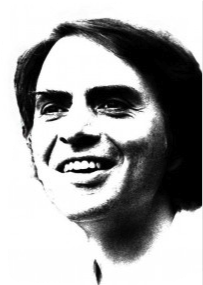
\includegraphics[width=\textwidth]{../figs/sagan.png}};
\end{tikzpicture}
\end{columns}
	\end{frame}
}

\section{Introduction}
\begin{ftst}
  {What is science?}
  {Some common misconceptions}

\bitem\item Science is a collection of facts; {\color{red}$\times$}
\item Science is the creation of new gadgets; {\color{red}$\times$}
\item Scientific ideas are absolute and unchangeable; {\color{red}$\times$}
\item Scientific ideas are subject to change, therefore unreliable; {\color{red}$\times$}
\item Observations give answers directly to the scientists; {\color{red}$\times$}
\item Science \textbf{proves} stuff; {\color{red}$\times$}
\item Science can only \textbf{disprove} stuff; {\color{red}$\times$}
\item The scientist works to \textbf{show} that his/her theory is right;{\color{red}$\times$}
\vone
\item \textbf{Theory} \textit{versus} \textbf{Law}.
\eitem
\let\thefootnote\relax\footnote{\scriptsize\textbf{Essential} reading: Common Misconceptions About Science: \url{http://goo.gl/TN7k9B}}
\begin{tikzpicture}[remember picture,overlay]
\node[anchor=north east,yshift=-34pt,xshift=0pt] at (current page.north east) {
\includegraphics[height=2cm]{../figs/xkcd_science.jpg}};
\node[anchor=north east,xshift=-5pt,yshift=-88pt] at (current page.north east) {\tiny \textbf{(http://xkcd.com)}};
\end{tikzpicture}
\end{ftst}

\begin{ftst}
 {What is science?}
  {Common methodological errors}
\bitems Personal biases (explicit or subtle);
	\item Premature conclusions;
	\item Confusion between concepts such as:
	\bitems conjecture;
	\item hypothesis;
	\item model;
	\item theory;\eitem
	\item Cherrypicking;
	\item Anomaly hunting;
	\item Anecdotal evidence;
\eitem
\end{ftst}

\begin{ftst}
  {What is science?}
  {The scientific process}
  
  \begin{columns}[T]
    \column{0.5\textwidth}
    \bitems Normally showed as a flowchart or a sequence of steps;
    \item Oversimplification of a complex and iterative process;
    \item Suggests that the process has an ``end''.
    \eitem
    \column{0.5\textwidth} 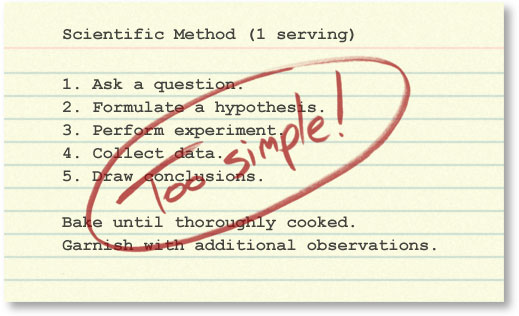
\includegraphics[width=\textwidth]{../figs/sciproc01.jpg}
  \end{columns}
  \vone
  \begin{columns}[T]
    \column{1.02\textwidth}
  \bitems The scientific process actually includes:
  \bitems Several activities, performed in different stages;
      \item Interaction with the scientific community;
      \item Creative, ``outside the box'' thinking;
      \item Preliminary conclusions, subject to revision as new and better data become available.
      \eitem\eitem
      \end{columns}
\begin{tikzpicture}[remember picture,overlay]
\node[anchor=south east,yshift=102pt, xshift=-10pt] at (current page.south east) {\tiny \url{http://goo.gl/7cCGaz}};
\node[anchor=south east,yshift=108pt, xshift=-10pt] at (current page.south east) {\tiny (c) Understanding Science, 2014. Used with permission.};
\end{tikzpicture}
\end{ftst}

\begin{ftst}
  {What is science?}
  {The scientific process}
\begin{center}
\vspace{-1.3em}
  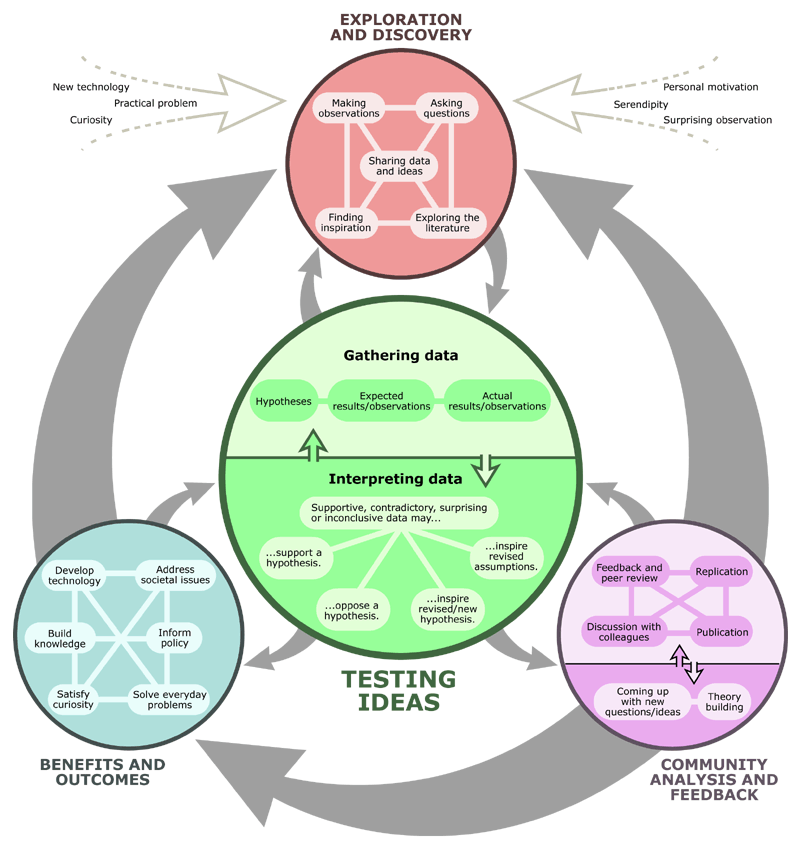
\includegraphics[width=0.64\textwidth]{../figs/sciproc02.png}
\end{center}
\begin{tikzpicture}[remember picture,overlay]
\node[anchor=south east,yshift=-2pt, xshift=0pt] at (current page.south east) {\tiny (c) Understanding Science, 2014. Used with permission.  \url{http://goo.gl/VglXc5}};
\end{tikzpicture}
  \end{ftst}
  
\begin{ftst}
  {What is science?}
  {The scientific process}
  \vspace{-1em}
  \begin{block}{}
``\textit{Dans les champs de l'observation le hasard ne favorise que les esprits pr�par�s.}'' -- \textbf{Louis Pasteur} (Univ. Lille, France, 1854).
  \end{block}
    \vskip -0.5em
  \begin{columns}[T]
    \column{0.45\textwidth}
  	\bitems Observation generating new \textbf{questions};
  	\item Exploratory experimentation;
  	\item The role of the pair\\preparation + serendipity.
	\eitem
    \column{0.55\textwidth} 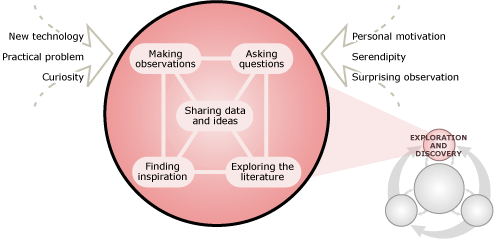
\includegraphics[width=\textwidth]{../figs/sciproc02a.png}
  \end{columns}
\vhalf
\begin{columns}[T]
    \column{0.3\textwidth}
    \begin{block}{\footnotesize Kekule (1865)}
\centering\includegraphics[width=0.35\textwidth]{../figs/kekule2.png}\\\small Structure of Benzene
    \end{block}
    \column{0.02\textwidth}
    \column{0.3\textwidth}
    \begin{block}{\footnotesize Becquerel (1896)}
\centering\includegraphics[width=0.38\textwidth]{../figs/becquerel2.png}\\\small Radioactivity
    \end{block}
    \column{0.02\textwidth}
    \column{0.3\textwidth}
    \begin{block}{\footnotesize Fleming (1928)}
\centering\includegraphics[width=0.37\textwidth]{../figs/fleming2.png}\\\small Penicillin
    \end{block}
    \column{0.01\textwidth}
    \end{columns}
  \begin{tikzpicture}[remember picture,overlay]
  \node[anchor=south east,yshift=96pt, xshift=-5pt] at (current page.south east) {\tiny (c) Understanding Science, 2014. Used with permission.};
  \node[anchor=south east,yshift=90pt, xshift=-5pt] at (current page.south east) {\tiny \url{http://goo.gl/fy8Glh}};
  \end{tikzpicture}

\end{ftst}


\begin{ftst}
  {What is science?}
  {The scientific process}
\bitems Drawing and testing hypotheses;
\item Comparing alternative explanations;
\item Accepting / rejecting ideas based on \textbf{evidence};
\item \textbf{Predictions} \textit{versus} \textbf{observation}: corroboration or refutation?
\eitem

  \begin{tikzpicture}[remember picture,overlay]
  \node[anchor=south,yshift=0, xshift=20pt] at (current page.south) {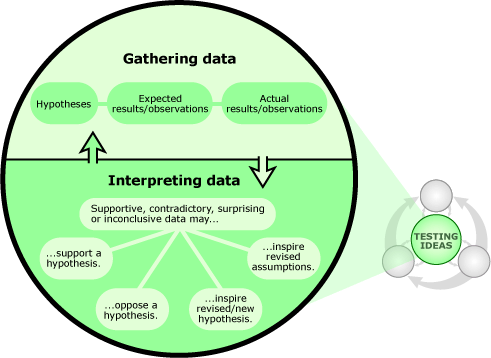
\includegraphics[width=0.6\textwidth]{../figs/sciproc02b.png}};
    \node[anchor=south east,yshift=8, xshift=-5pt] at (current page.south east) {\tiny \url{http://goo.gl/aOgSqT}};
    \node[anchor=south east,yshift=0, xshift=-5pt] at (current page.south east) {\tiny (c) Understanding Science, 2014. Used with permission.};
  \end{tikzpicture}
\end{ftst}


\begin{ftst}
  {What is science?}
  {The scientific process}
  \vspace{-0.4em}
\begin{columns}[T]
    \column{0.75\textwidth}
\textbf{James Lind} (1747):\\
\bitems Conjecture: Scurvy was caused by the rottenness of the body;
\item Idea: try to avoid/reverse its effects with acidic substances;\eitem
  \column{0.25\textwidth}
\end{columns}
\vone
Separation of a group of 12 sailors with scurvy in six groups. Identical diets, except for the addition of a supplement:
\begin{columns}[T]
    \column{0.30\textwidth}
\begin{colorblock}{Group 1}{bg=green!30,fg=black}
\small Cider.
\end{colorblock}
\begin{block}{Group 4}
\small Sea water.
\end{block}
    \column{0.30\textwidth}
\begin{block}{Group 2}
\small Vitriol.
\end{block}
\begin{colorblock}{Group 5}{bg=green!90,fg=black}
\small Oranges and lemons.
\end{colorblock}
    \column{0.30\textwidth}
\begin{block}{Group 3}
\small Vinegar.
\end{block}
\begin{block}{Group 6}
\small Tea.
\end{block}
    \end{columns}
  \begin{tikzpicture}[remember picture,overlay]
  \node[anchor=north east,yshift=-38, xshift=-25pt] at (current page.north east) {\includegraphics[width=2.2cm]{../figs/lind2.png}};
  \end{tikzpicture}
\end{ftst}


\begin{ftst}
  {What is science?}
  {The scientific process}
  \begin{columns}[T]
    \column{0.5\textwidth}
  	\bitems Interaction with the scientific community is \textbf{essential}:
  	\bitems Colleagues;
  	\item Collaborators;
  	\item Reviewers;
  	\item Rivals;\eitem
	\eitem
    \column{0.5\textwidth}   \vskip -1em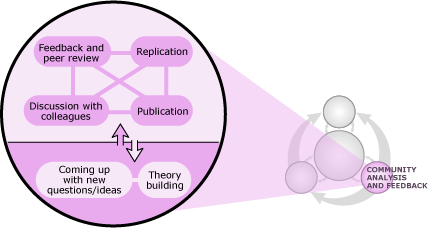
\includegraphics[width=\textwidth]{../figs/sciproc02c.png}
  \end{columns}
\vone
  \begin{columns}[T]
    \column{1.02\textwidth}
 \bitems This interaction plays essential roles to the progress of research:\eitem
    \end{columns}
    \vhalf
\begin{columns}[T]
    \column{0.22\textwidth}\begin{block}{Criticism}
\centering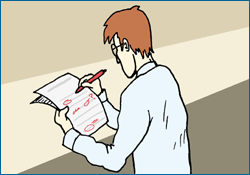
\includegraphics[width=\textwidth]{../figs/community2.png}
    \end{block}
    \column{0.22\textwidth}\begin{block}{Inspiration}
\centering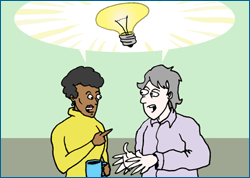
\includegraphics[width=\textwidth]{../figs/community3.png}
        \end{block}
    \column{0.22\textwidth}\begin{block}{Vigilance}
\centering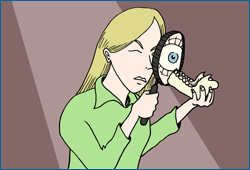
\includegraphics[width=\textwidth]{../figs/community4.png}
        \end{block}
    \column{0.22\textwidth}\begin{block}{Motivation}
\centering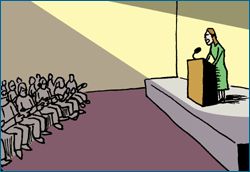
\includegraphics[width=\textwidth]{../figs/community5.png}
        \end{block}
    \end{columns}
  \begin{tikzpicture}[remember picture,overlay]
  \node[anchor=south east,yshift=0pt, xshift=-5pt] at (current page.south east) {\tiny (c) Understanding Science, 2014. Used with permission. \url{http://goo.gl/9pSCTG}};
  \end{tikzpicture}

\end{ftst}

\begin{ftst}
  {What is science?}
  {The scientific process}
\bitems Publication and peer review\eitem
\begin{columns}[T]
    \column{0.5\textwidth}
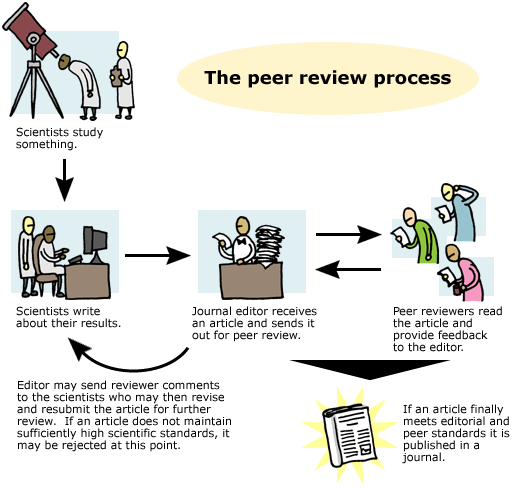
\includegraphics[width=1.15\textwidth]{../figs/peerreview.png}
    \column{0.5\textwidth}
    \bitems Additionally,  \textbf{post-publication} review;
    \spitem \textbf{Replication} and verification of the results by researchers in the same field;
    \spitem Importance of \textbf{replicability} of the work.
    \eitem
    \end{columns}
  \begin{tikzpicture}[remember picture,overlay]
  \node[anchor=south west,yshift=8pt, xshift=5pt] at (current page.south west) {\tiny  \url{http://goo.gl/VWCVkK}};
  \node[anchor=south west,yshift=0pt, xshift=5pt] at (current page.south west) {\tiny (c) Understanding Science, 2014. Used with permission.};
  \end{tikzpicture}

\end{ftst}



\begin{ftst}
  {What is science?}
  {The scientific process}
  \begin{columns}[T]
    \column{0.55\textwidth}
  	\bitems The scientific process is a way of building knowledge:
  	\bitems Generation and testing of new ideas about how the world works;
    \item Iterative increase in the reliability of results;\eitem
	\eitem
    \column{0.45\textwidth}   \vskip -1em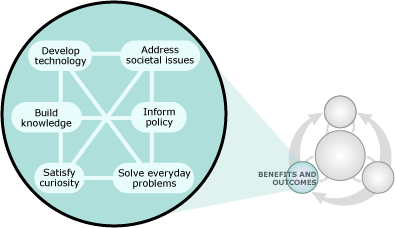
\includegraphics[width=\textwidth]{../figs/sciproc02d.png}
  \end{columns}
\vhalf
  \begin{columns}[T]
    \column{0.32\textwidth}\begin{block}{}
\centering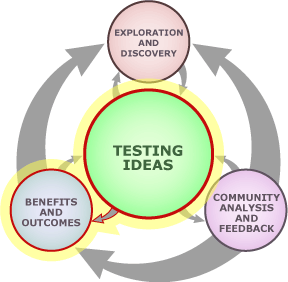
\includegraphics[width=0.9\textwidth]{../figs/benefitschart1.png}\\
\scriptsize Knowledge$\rightarrow$Applications
    \end{block}
    \column{0.32\textwidth}\begin{block}{}
\centering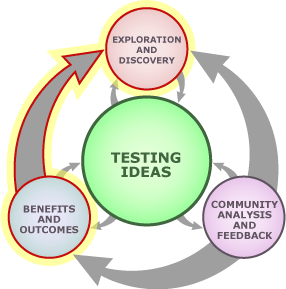
\includegraphics[width=0.88\textwidth]{../figs/benefitschart2.png}\\
\scriptsize Technologies$\rightarrow$Discovery
        \end{block}
    \column{0.32\textwidth}\begin{block}{}
\centering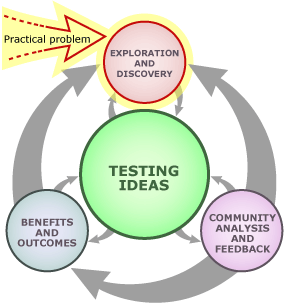
\includegraphics[width=0.85\textwidth]{../figs/benefitschart3.png}\\
\scriptsize Applications$\rightarrow$Investigation
        \end{block}
    \end{columns}
  \begin{tikzpicture}[remember picture,overlay]
  \node[anchor=south east,yshift=132pt, xshift=-5pt] at (current page.south east) {\tiny  \url{http://goo.gl/IBRSoQ}};
   \node[anchor=south east,yshift=124pt, xshift=-5pt] at (current page.south east) {\tiny (c) Understanding Science, 2014. Used with permission.};
  \end{tikzpicture}
\end{ftst}

\begin{ftst}
{What is science?}
{To wrap it up}
\vskip 4em
\begin{columns}[T]
    \column{0.8\textwidth}
\flushright{\small ``\textit{
It is important to be literate in the scientific method,\\
not only for the sake of your own research. We are also\\
agents of change in the population and, as such, we need\\
to be aware of good and bad science, and able to point the\\
difference to the society.}''\\\ \\\small Claus Aranha, 2013\\Tsukuba University}
\column{0.2\textwidth}
\begin{tikzpicture}[remember picture,overlay]
\node[anchor=south east,yshift=62pt,xshift=0pt] at (current page.south east) {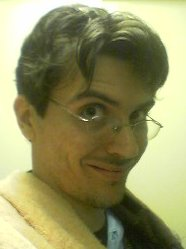
\includegraphics[width=\textwidth]{../figs/caranha.png}};
\end{tikzpicture}
\end{columns}
\end{ftst}



\begin{ftst}
{Experiments}
{Definition of experiment}
\vskip 6em
\begin{block}{}
\begin{center}
\textit{A test (or a series of tests) where changes are introduced in the state of a system or process, enabling the observation and characterization of effects that can occur resulting from these changes.}
\end{center}
\end{block}
\end{ftst}

\begin{ftst}
{Experiments}
{Objectives of experiments}
\bitems To determine which variables are more influential in a given system or process;
\spitem To determine desired values for parameters of the system to:
\vhalf
\bitems Obtain desired output values;
\item Minimize output variability;
\item Minimize the effects of external factors;
\eitem
\spitem Characterize behavior of the system or process under study.
\eitem
\end{ftst}

\begin{ftst}
{Experiments}
{Data gathering}
\begin{block}{}
\begin{itemize}
{\small\item\alert{Retrospective study};
\item Observational study;
\item Designed experiment;}
\end{itemize}
\end{block}
\begin{block}{Characteristics}
{\small\bitems Use of historical data;
\item Investigating correlations;\eitem
}
\end{block}
\begin{block}{Problems}
{\small\bitems Data representativeness;
\item Availability of data;\eitem
}
\end{block}

\end{ftst}

\begin{ftst}
{Experiments}
{Data gathering}
\begin{block}{}
\begin{itemize}
{\small\item Retrospective study;
\item \alert{Observational study};
\item Designed experiment;}
\end{itemize}
\end{block}
\begin{block}{Characteristics}
{\small\bitems Observation of the system with minimal disturbance;
\item Investigation of usual behaviors;\eitem
}
\end{block}
\begin{block}{Problems}
{\small\bitems Low representativeness of extreme cases;
\item Low variability can affect observation of interesting effects;\eitem
}
\end{block}
\end{ftst}


\begin{ftst}
{Experiments}
{Data gathering}
\begin{block}{}
\begin{itemize}
{\small\item Retrospective study;
\item Observational study;
\item \alert{Designed experiment};}
\end{itemize}
\end{block}
\begin{block}{Characteristics}
{\small\bitems Introduction of deliberate changes in the system;
\item Inference on the \textit{causality} of the effects;\eitem
}
\end{block}
\begin{block}{Problems}
{\small\bitems Requires rigorous experimental design and data analysis;
\item May need greater sample sizes.\eitem
}
\end{block}
\end{ftst}

\begin{ftst}
{Experimentation strategies}
{Educated guess}
\vspace{-1em}
\begin{columns}[T]
    \column{1.02\textwidth}
\begin{block}{}
\bitems Select arbitrary combination of levels for the factors;
\item Test and observe behavior; 
\item Change one or two factors at a time, then re-test;\eitem
\end{block}
\bitems Widely used in engineering;
\item Can achieve good results, but has a lot of limitations;
\eitem
%\centering\includegraphics[width=0.8\textwidth]{../figs/edguess1.png}
\end{columns}
\end{ftst}

\begin{ftst}
{Experimentation strategies}
{Educated guesses}
\vspace{-1em}
\begin{columns}[T]
    \column{0.79\textwidth}
    \begin{block}{}
    \bitems Select arbitrary combination;
    \item Test an observe; 
    \item Change and re-test;\eitem
    \end{block}
    \vone
\centering
\includegraphics[width=0.75\textwidth]{../figs/edguess3.png}
    
    \column{0.21\textwidth}
\centering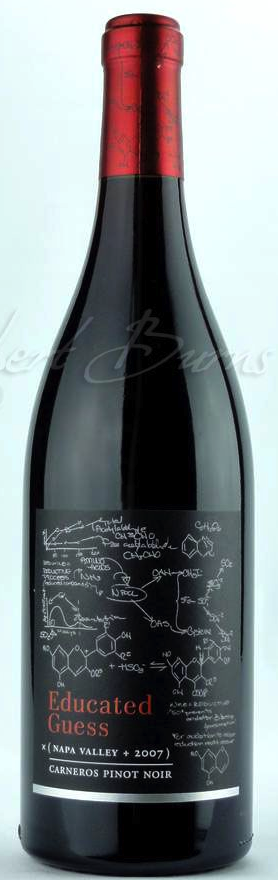
\includegraphics[width=\textwidth]{../figs/edguess2.png}
\end{columns}
\end{ftst}

\begin{ftst}
{Experimentation strategies}
{Educated guesses}
\vspace{-1em}
\begin{columns}[T]
    \column{0.79\textwidth}
    \begin{block}{}
    \bitems Select arbitrary combination;
    \item Test an observe; 
    \item Change and re-test;\eitem
    \end{block}
    \vone
\centering
\includegraphics[width=0.75\textwidth]{../figs/edguess3.png}
    
    \column{0.21\textwidth}
\centering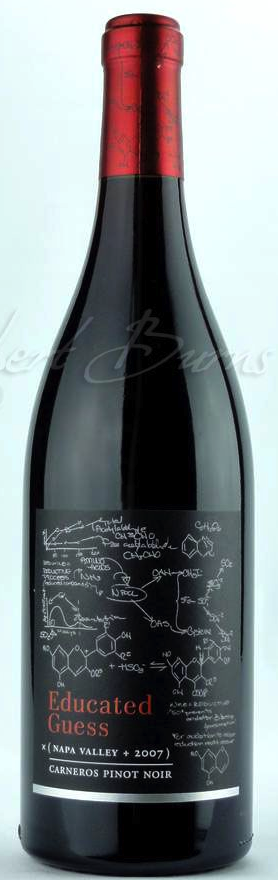
\includegraphics[width=\textwidth]{../figs/edguess2.png}
\end{columns}
\begin{tikzpicture}[remember picture,overlay]
  \node[anchor=south,yshift=25pt, xshift=0pt] at (current page.south) {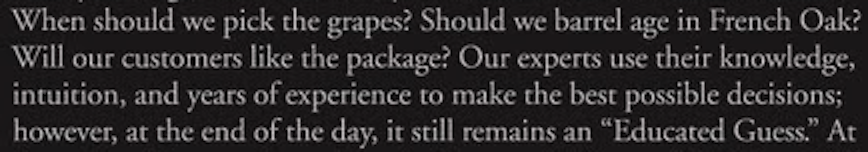
\includegraphics[width=12cm]{../figs/edguess3b.png}};
  \end{tikzpicture}
\end{ftst}


\begin{ftst}
{Experimentation strategies}
{One factor at a time}
\begin{columns}[T]
    \column{1.02\textwidth}
\begin{block}{}
\begin{itemize}
\item Select one reference point;%(point?)
\item Change each factor individually, keeping the others constant;
\end{itemize}
\end{block}

\bitems Widely used in practice (particularly in algorithm research);
\item Good results when there are no interaction effects;
\eitem
\end{columns}
\begin{tikzpicture}[remember picture,overlay]
  \node[anchor=south east,yshift=0pt, xshift=-5pt] at (current page.south east) {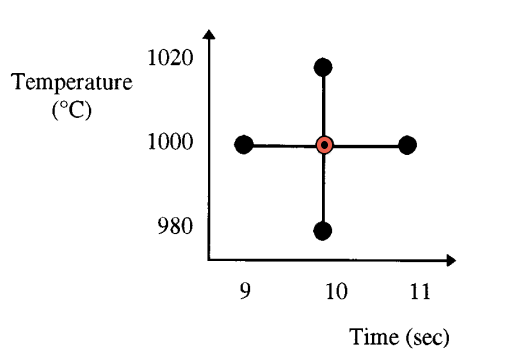
\includegraphics[width=5.5cm]{../figs/OFAT01c.png}};
  \end{tikzpicture}
\end{ftst}

\begin{ftst}
{Experimentation strategies}
{Factorial designs}
\begin{columns}[T]
    \column{1.02\textwidth}
\begin{block}{}
\begin{itemize}
\item Select \textbf{levels} for each factor;
\item Vary the factors simultaneously, in a systematic way;
\end{itemize}
\end{block}
\bitems Estimation of main effects and interactions;
\item Greater precision in the effect estimates;
\item More efficient use of resources (information/observation);
\eitem
\end{columns}
\begin{tikzpicture}[remember picture,overlay]
  \node[anchor=south east,yshift=0pt, xshift=-5pt] at (current page.south east) {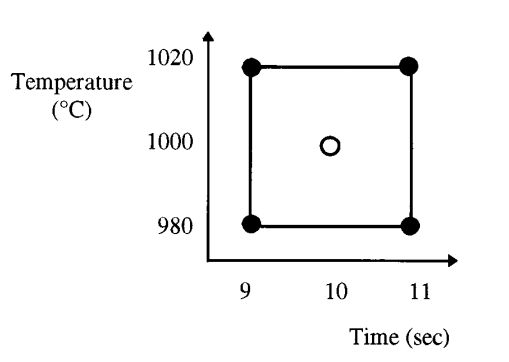
\includegraphics[width=5.5cm]{../figs/FFD01a.png}};
  \end{tikzpicture}
\end{ftst}

\section{Fundamental principles}
\begin{ftst}
{Fundamental principles}
{Design of experiments (DoE)}
\vone
\begin{block}{}
\textit{Process of designing data gathering protocols to enable accurate data analyses by statistical tools, capable of supporting sound and objective conclusions.}
\end{block}

\bitems Applicable to any system or process subject to noise, experimental errors, etc.
\item Necessary for the conclusions to have \textbf{statistical meaning};
\item Helps avoiding errors due to personal biases, besides other artifacts of experimentation and analysis.
\eitem
\end{ftst}

\begin{ftst}
{Fundamental principles}
{Design of experiments (DoE)}
\begin{block}{Design of the experiment}
\small
\bitems Scientific/technical question of interest;
\item Selection of factors and levels;
\item Sample size calculations;
\item Determination of protocols for data gathering;
\eitem
\end{block}
\begin{block}{Statistical analyses of the data}
\small
\bitems Definition of the desired confidence level;
\item Definition and calculation of the test statistic;
\item Validation of the assumptions of the statistical model;
\item Calculation of the magnitude of effects;
\item Drawing of conclusions and recommendations;
\eitem
\end{block}
\end{ftst}

\begin{ftst}
{Fundamental principles}
{Design of experiments (DoE)}
\begin{block}{}
\bitems \alert{Repetition e replication};
\item Randomization;
\item Blocking;\eitem %(?????)
\end{block}
\bitems Repeated measurements - estimation of the variability intra-groups;
\item Replication - estimative of the experimental error;
\item Greater precision in the model terms;
\eitem
\centering\includegraphics[width=.65\textwidth]{../figs/2x2DoE-replic.png}
\end{ftst}


\begin{ftst}
{Fundamental principles}
{Design of experiments (DoE)}
\begin{block}{}
\bitems Repetition e replication;
\item \alert{Randomization};
\item Blocking;\eitem %(?????)
\end{block}
\bitems Avoids contamination of the data by order-dependent effects (time, position, etc.);
\vhalf
\bitems Heating effects;
\vhalf
\item Wear and tear effects;
\vhalf
\item External interferences;\eitem
\eitem
\end{ftst}

\begin{ftst}
{Fundamental principles}
{Design of experiments (DoE)}
\begin{block}{}
\bitems Repetition e replication;
\item Randomization;
\item \alert{Blocking};\eitem %(?????)
\end{block}
	\bitems Improvement in the estimation of effects for the factors of interest;
	\spitem Reduction or eliminations of inconvenient factor effects (ones that influence the response, but are not interesting for the analyses)
\eitem
\vone
\begin{colorblock}{}{bg=green!70,fg=black}
\centering Example: effects of different measurement equipments.
\end{colorblock}
\end{ftst}


\begin{ftst}
{Fundamental principles}
{The role of experimental design}
\begin{itemize}
    \item Avoiding the influence of spurious factors and personal biases;
	\item Perform experiments in a impartial and objective way.
\end{itemize}
\vone
\begin{block}{}
\vhalf
\centering``\textit{Never have too much love for your hypotheses.}''
\vspace{0.5em}
\end{block}
\vone
\begin{columns}[T]
    \column{0.3\textwidth}\ 
    \column{0.7\textwidth}
\begin{block}{}
\flushright``\textit{The great tragedy of Science - the slaying of a\\
\vspace{-1em}\flushright beautiful hypothesis by an ugly fact.}''\\
\flushright Thomas H. Huxley (1870)
\vspace{0.5em}
\end{block}
\end{columns}

\begin{tikzpicture}[remember picture,overlay]
  \node[anchor=south west,yshift=15pt, xshift=10pt] at (current page.south west) {\tiny \textbf{Source}: \url{http://goo.gl/y4H7nj}};
  \node[anchor=south west,yshift=20pt, xshift=25pt] at (current page.south west) {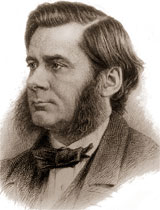
\includegraphics[width=2.5cm]{../figs/huxley.png}};
  \end{tikzpicture}
\end{ftst}

\begin{ftst}
{Example}
{Jacques Benveniste and the memory of water}
\begin{columns}
\column[T]{0.8\textwidth}
\begin{itemize}
	\item Published in Nature (1988);
	\item Investigation: Maddox, Stewart, Randi;
	\item Introduction of blinding into the experiment\\- the effect disappears!
\end{itemize}
\column[T]{0.2\textwidth}
\begin{tikzpicture}[remember picture,overlay]
\node[anchor=north east,yshift=-50pt, xshift=-10pt] at (current page.north east) {\includegraphics[width=\textwidth]{../figs/benveniste2.png}};
  \end{tikzpicture}
\end{columns}
\vone\vone
Methodological problems in design and analysis:
\begin{columns}
\column[T]{0.8\textwidth}
\begin{block}{}
\small
\bitems No blinding - experimenter bias;
		\item Cherrypicking;
		\item Contamination;
		\item Incorrect statistical analysis;
		\item Non-reproducibility;
\eitem
\end{block}
\column[T]{0.2\textwidth}
\end{columns}
\end{ftst}


\section{Structure of Experimental Design}
\begin{ftst}
{Structure of Experimental Design}
{Main points}
To enable the use of a scientific approach in the experimental design, it is necessary to understand:
\vhalf
\begin{itemize}
	\item The field where the experiment is to be conducted;
	\vhalf
	\item The strategy for data collection;
	\vhalf
	\item The way the data should be analyzed (at least qualitatively).
\end{itemize}
\end{ftst}

\begin{ftst}
{Structure of Experimental Design}
{Guidelines for a good design}
\bitems Pre-experimental design:\begin{enumerate}[(a)]
		\item Identification and definition of the problem;
		\item Choice of factors of interest, levels, ranges;
		\item Selection of the response variable (or variables);
	\end{enumerate}
	\spitem Choice of the experimental design;
	\spitem Conduction of the experiment;
	\spitem Statistical data analyses;
	\spitem Conclusions and recommendations;
\eitem
\end{ftst}

\begin{ftst}
{Pre-experimental design}
{Before we start...}
\bitems Is the investigation relevant?
\spitem Would the results be interesting for the research community?
\spitem Practical relevance?
\bitems Employ exploratory experiments;\eitem
\spitem Placement within the literature;
\bitems Avoid repetition and irrelevance.\eitem
\eitem
\vspace{35pt}
\begin{block}{}
{\ \\\ \\\scriptsize``\textit{Sometimes one should do a completely wild experiment,\\like blowing the trumpet to the tulips every morning\\for a month. Probably nothing would happen, but what if it did?}''\\}
{\tiny -- Sir George Howard Darwin}
\end{block}
\begin{tikzpicture} [remember picture,overlay]
\node[anchor=south east,yshift=5pt,xshift=10pt] at (current page.south east) {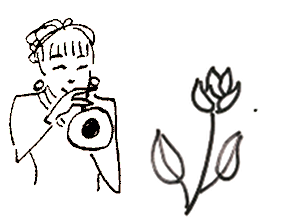
\includegraphics[height=2.5cm]{../figs/ttt.png}};
\end{tikzpicture}
\end{ftst}

\begin{ftst}
{Pre-experimental design}
{Definition of hypotheses}
\bitems Exploratory experimentation $\neq$ careless experimentation;
\spitem Data collection guided by questions of interest;
\bitems Difference on average/best/worst performance;
\spitem Robustness / reliability;
\eitem
\spitem The translation \textit{scientific question} $\rightarrow$ \textit{test hypothesis} requires special attention, and a solid knowledge of the technical area in which the experiment is being performed;
\eitem
\end{ftst}


\begin{ftst}
{Choice of Experimental Design}
{Experimental design}
\begin{itemize}
	\item (Relatively) simple, as long as the pre-experimental part is well done;
	\spitem Dependent on what is being tested (statistical question);
	\spitem A sound design tends to determine the analyses technique to be used, at least  qualitatively;
	\spitem Involves considerations about:\begin{itemize}
	\item Sample size;
	\item Ordering of observations;
	\item Determination of restrictions to the randomization and the use of blocks, etc.
\end{itemize}
\spitem Available in several statistical/mathematical packages;
\end{itemize}
\end{ftst}

\begin{ftst}
{Choice of Experimental Design}
{Problem-dependent}
\bitems Depending on the experimental question, different experimental designs are required
\spitem A solid, statistically sound design tends to determine which statistical tests must be employed in the analysis step, at least qualitatively.
\spitem Determination of the proportion of between-groups and within-groups variability;\eitem
\end{ftst}

\begin{ftst}
{Realization of Experiments}
{Data gathering}
\bitems Must be consistent with design, otherwise the validity of the results may be compromised - data collection must always follow the plan:\vhalf
\bitems No premature stops;\vhalf
	\item \textit{No-peeking rule};\eitem

\spitem Use of pilot experiments:\vhalf
\bitems Gathering of preliminary information;\vhalf 
\item Practice with the experimental conditions;
\eitem\eitem
\end{ftst}

\begin{ftst}
{Analysis of the experimental data}
{A consequence of design}
\bitems Analyses techniques are (mostly) simple, but the devil is in the details.
\spitem Use of existing statistical tools and frameworks, such as\eitem
\begin{center}
\includegraphics[width=0.2\textwidth]{../figs/rlogo.png}
\end{center}
\bitems Free, versatile, good graphical capabilities, relatively simple;
\eitem
\end{ftst}

\begin{ftst}
{Analysis of the experimental data}
{Statistical modeling}
\bitems General procedure for testing the experimental hypotheses:
\bitems Definition of a \textit{null-model} (absence of effects) and of a desired level of significance;
\spitem Determination of $P(data|\mbox{\textit{null-model}})$;
\spitem Decision by rejection (or not) of the null hypothesis;
\spitem Validation of model assumptions;
\spitem Estimation of the  \textit{magnitude} of differences - \textbf{practical significance};
\eitem\eitem

\begin{block}{}
\centering\textit{Statistical methods do not \textbf{prove} anything, but they allow an objective definition of margins of plausibility for certain statements.}
\end{block}\end{ftst}

\begin{ftst}
{Reporting of results}
{Presentation}
\bitems Combine textual, numeric and graphical elements to tell a story with your data.
\bitems Simplifies understanding and analysis of the results\eitem
\spitem Strive to achieve graphical excellence;
\bitems (E. Tufte: \textit{The Visual Display of Quantitative Information})
\item(N. Yau, Visualize This!)\eitem
\spitem Coherence of notation - special attention to figures and tables;
\spitem Display simultaneous confidence intervals and other graphical indicators of effect size.
\eitem
\begin{tikzpicture} [remember picture,overlay]
\node[anchor=south east,yshift=110pt,xshift=3pt] at (current page.south east) {
\includegraphics[height=2.5cm]{../figs/tufte.png}};
\end{tikzpicture}

\end{ftst}

\begin{ftst}
{Conclusions}
{Drawing and reporting conclusions}
\bitems Conclusions should be based on solid evidence from the data;
\spitem Be conservative - it is common to exaggerate the generality of the results;
\spitem Report significance levels and the assumptions under which the results are valid;
\spitem \textit{Suggest explanations} to the observed results;
\spitem Careful with \textit{anomaly hunting};\eitem

\begin{block}{}
\small\textit{Always let the science drive the statistics. If you get a statistically significant result, go back and describe what it means in the scientific context.}
\flushright\footnotesize Aaron Rendahl (2010)
\end{block}
\end{ftst}

\begin{ftst}
{Discussion}
 {Some more relevant points}
\bitems Use of previous knowledge, theoretical or empirical;
\spitem Iterative experimentation;
\spitem Statistical experimentation$\times$ practical significance;
\spitem Use of additional experiments to validate conclusions.
\eitem
\end{ftst}


\section{Bibliography}
{ 
\begin{ftst}
{Bibliography}
{References used}
\footnotesize
\begin{enumerate}
	\item D.C. Montgomery, \textit{Design and Analysis of Experiments}, 5th ed., Wiley, 2005;
	\item J.S. Kim, J.W. Kalb, \textit{Design of Experiments: An Overview and Application Example} - \url{http://goo.gl/iP08X}
	\item J. Trygg, \textit{Introduction to Statistical Experimental Design} \url{http://goo.gl/zrScf}
	\item \textit{Understanding Science}. 2014. University of California Museum of Paleontology. 3 January 2014  \url{http://www.understandingscience.org}
	\item V. Czitron, \textit{One-Factor-at-a-Time Versus Designed Experiments}, The American Statistician, 53(2) 126-131, 1999.
	\item A. Rendahl, \textit{Experimental design and statistical analysis: questions to consider as you write your grant} - \url{http://goo.gl/yT0TK7}
\end{enumerate}
\end{ftst}

\begin{ftst}
{Bibliography}
{Recommended literature}
\footnotesize
\begin{enumerate}
	\item Carl Sagan,\textit{The demon-haunted world: science as a candle in the dark},\\Random House, 1996.
	\item T. Brady, \textit{Reviewer's quick guide to common statistical errors in scientific papers}\\\url{http://goo.gl/96Qfk}
	\item F.L.H. Wolfs, \textit{APPENDIX E: Introduction to the Scientific Method}. \url{http://goo.gl/osGpU}
	\item Dept. Biochemistry \& Cell Biology, Rice University , \textit{Common Errors in Student Research Papers}. \url{http://goo.gl/FPDBj}
	\item B. Dunning, \textit{An Enthusiast's Primer on Study Types}. Skeptoid Podcast, Skeptoid Media, Inc., 2013. - \url{http://skeptoid.com/episodes/4381}
	\item J. Maddox, J. Randi, and W.W. Stewart, \textit{``High-dilution'' experiments a delusion}, Nature 334, 287-290, 1988
	\item Science blogs - Bad Astronomy, The Skeptics Guide to the Universe, Science-Based Medicine, NeuroLogica, Planetary Radio, Radiolab, etc.	
\end{enumerate}
\end{ftst}
}

\begin{ftstf}{About this material}{Conditions of use and referencing}
\centering\footnotesize This work is licensed under the Creative Commons CC BY-NC-SA 4.0 license\\(Attribution Non-Commercial Share Alike International License version 4.0).\\
\vhalf
\url{http://creativecommons.org/licenses/by-nc-sa/4.0/}\\
\vone
Please reference this work as:\\
\flushleft Felipe Campelo (2014), \textit{Lecture Notes on Design and Analysis of Experiments}.\\Online: \url{http://www.ppgee.ufmg.br/~fcampelo/LNDoE/}.\\
Version 2.1, Ch. 1; Creative Commons BY-NC-SA 4.0.\\

\begin{Verbatim}[fontsize=\scriptsize]
    @Misc{Campelo2014,
      title={Lecture Notes on Design and Analysis of Experiments},
      author={Felipe Campelo},
      howPublished={\url{http://www.ppgee.ufmg.br/~fcampelo/LNDoE/}},
      year={2014},
      note={Version 2.1, Ch. 1; Creative Commons BY-NC-SA 4.0.},
    }
\end{Verbatim}

\begin{tikzpicture} [remember picture,overlay]
\node[anchor=south,yshift=0pt] at (current page.south){ \includegraphics[width=.2\textwidth]{../figs/CCSomerights.png}};
\end{tikzpicture}
\end{ftstf}


\begin{ftst}{About this material}{Acknowledgments}
Special thanks to:\\
\vhalf
\bitems Prof. Claus Aranha (Tsukuba University), for discussions and contributions to this material;
\spitem My M.Sc. student Fernanda Takahashi, for working on the English translation of the original slides;
\spitem Previous students from the Graduate Program in Electrical Engineering (PPGEE/UFMG), in particular Bernardo Braga and David Pinto, for pointing out errors and helping me improve these Lecture Notes.
\eitem
\end{ftst}

\end{document}